\documentclass{beamer}

%\usepackage[latin2]{inputenc}
%\usepackage[T1]{fontenc}
\usepackage{amsmath,amssymb} % AMS matematikai és fontcsomag
\usepackage{amsthm}          % tételszerű környezetek
\usepackage{graphicx}        % képek beillesztéséhez
\usepackage{geometry}        % méretek állítása
\usepackage{subcaption} 	 % subfigure
\usetheme{Antibes}
\useoutertheme{miniframes} % Alternatively: miniframes, infolines, split
\useinnertheme{circles}
\usecolortheme{beaver}

\newtheorem{thm}{Theorem}
\newtheorem{defi}[thm]{Definition}
\newtheorem{lem}[thm]{Lemma}
\newtheorem{cor}[thm]{Corollary}
\newtheorem{prop}[thm]{Proposition}
\newtheorem{rem}[thm]{Remark}

\def\IR{\mathbb{R}}
\def\IT{\mathbb{T}}
\def\IN{\mathbb{N}}
\def\IZ{\mathbb{Z}}
\def\SS{\mathbb{S}}


\title{Analyzing the evolution of the European Parliament Social Network}

\date{2023-11-10}

\author{Á. Bernát, M. Marits}

\usepackage{graphicx}

%\setbeamertemplate{background}{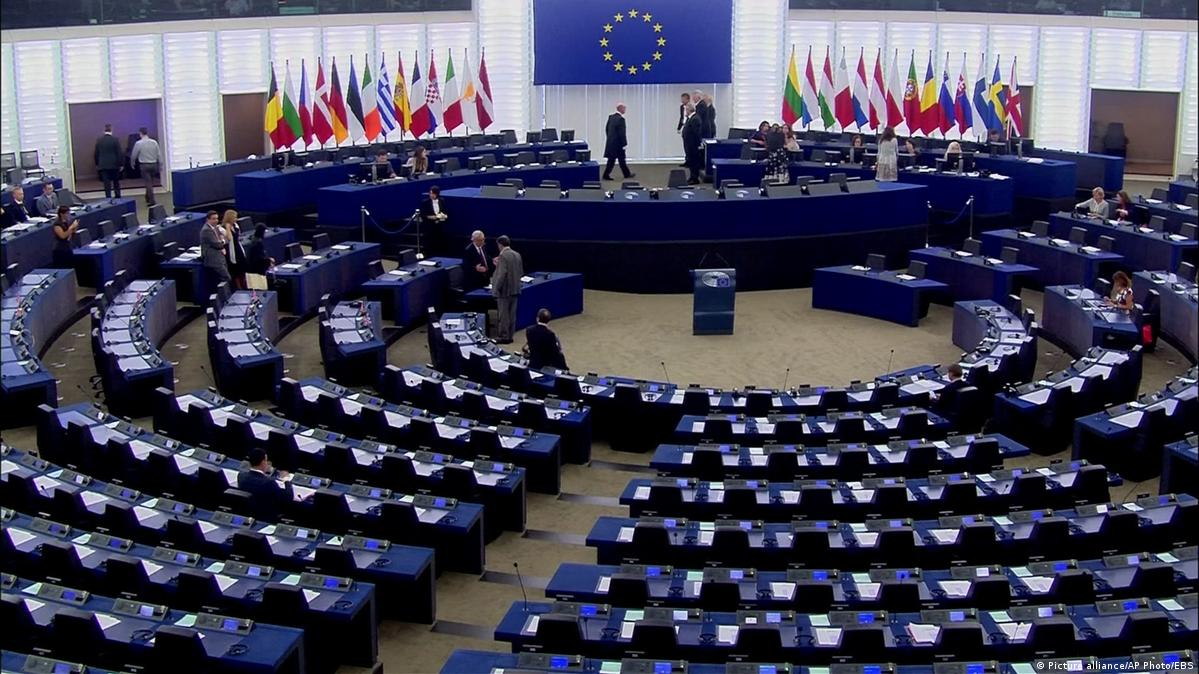
\includegraphics[width=\paperwidth,height=\paperheight,keepaspectratio]{img/euparl.jpg}}

\begin{document}
\begin{frame}[plain]
    \maketitle
\end{frame}

\begin{frame}{Introduction}
	
	\begin{figure}
		The European Parliament
	
		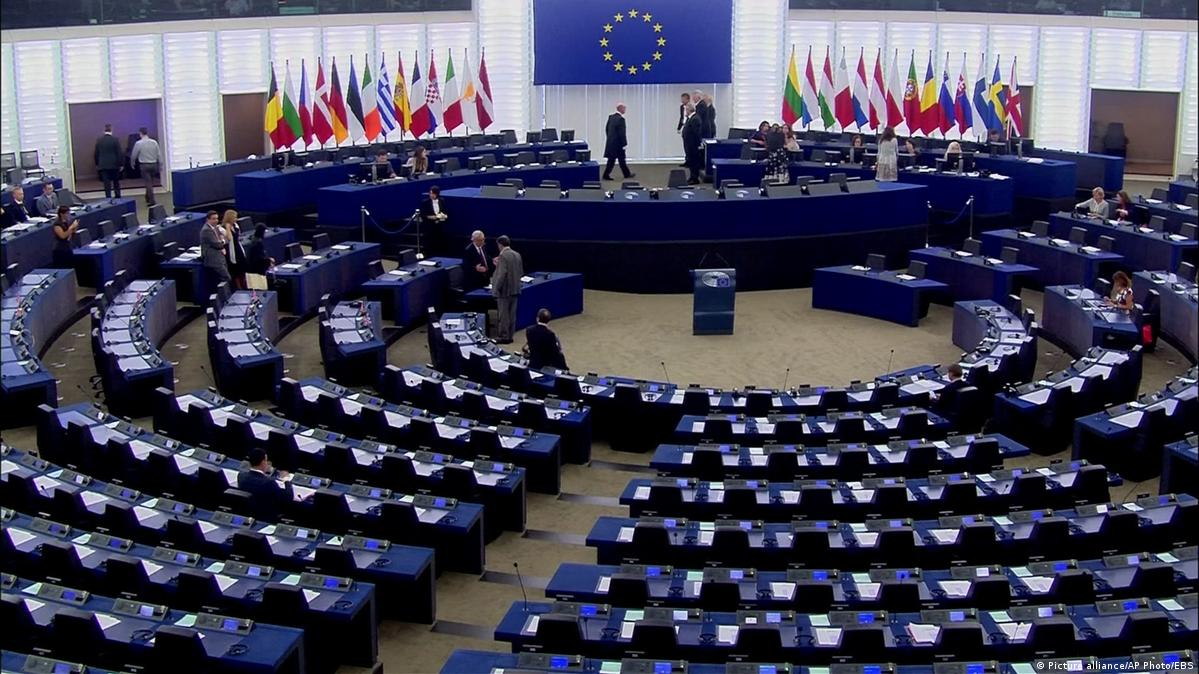
\includegraphics[width=0.5\textwidth]{img/euparl.jpg}
	\end{figure}

	We are analyzing a dataset of European Parliament members.
	
	\vspace{2mm}
	
	Our dataset is a list of ammendments.

	
\end{frame}

\begin{frame}
\frametitle{Our analysis}

\begin{columns}

\column{5cm}

We acquired data regarding amendments, for each amendment we know which MEP proposed the amendment, what kind of document it is, etc..
\bigskip

\pause Basically, we got a bipartite graph with node groups:
\begin{itemize}
	\item MEPs
	\item Documents
\end{itemize}
\bigskip

\pause Edges $\iff$ MEP made amendment to document

\pause \column{5cm}
\begin{center}
\small{A bipartite graph:}
\bigskip
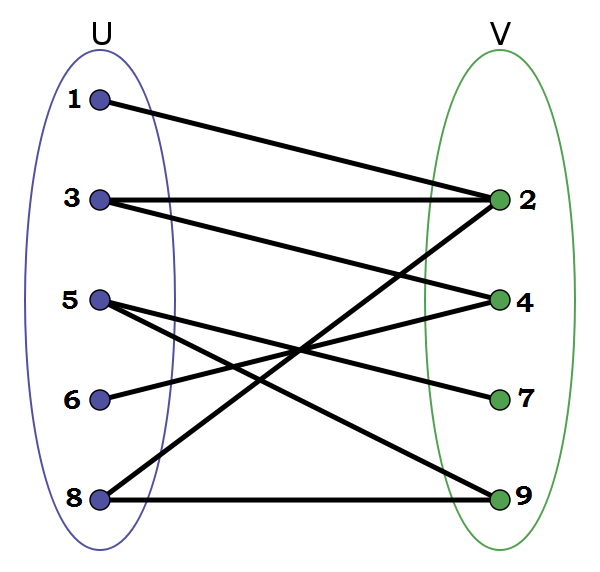
\includegraphics[height=3.2cm]{img/BipartiteGraph.png}
\end{center} 

\end{columns}
\end{frame}



\begin{frame}
\frametitle{Projection}

We then created a projection of this bipartite graph:

\begin{itemize}
	\pause \item Nodes: the nodes of MEPs
	\pause \item Edges: 2 MEPs are connected if they amended the same document	
\end{itemize}


%\pause We have also considered and implemented weighted projection. We used the so called: "Collaboration weighted projection"(where we reward secluded document matching and punish popular document matching)
%EZ nem tom kell e ? 

\end{frame}


\begin{frame}{Committees}

	HERE WHAT IS A COMMITTEE 
	\pause Commitee members work together on a specific set of law changes

	EG FOR COMMITTEES (ITRE, ENVI)
	\vspace{2mm}
	
	\pause We will also analyze the changes in the network based on the committees
	
\end{frame}

\begin{frame}
\frametitle{Motivation}

Understanding the network of MEPs might give us a better understanding of the following:

\bigskip

\begin{itemize}
	\pause \item How smaller networks inbetween MEPs look like, their size and their quantity.
	
	\pause \item \textbf{How events and occurrences shape the form and topology of the network.}
		
	\pause \item \textbf{How different groups behave within the network over time}

\end{itemize}

\pause All of these are helpful in understanding the processes regarding proposals and how they evolve into enacted laws.

\end{frame}

\begin{frame}{Analysis topic}
	
	We want to analyze the changes in the social network of the EP over time.
	
	\vspace{2mm}
	
	\pause For this, we picked two important properties of the network to investigate\begin{itemize}
		\pause \item Centrality of groups/MEPs
		
		\pause \item Cohesion of the network
	\end{itemize}
	
\end{frame}

\begin{frame}{Analyzing centrality in the network}
	
	Group centralities (similar to node centralities):
\begin{itemize}
	\pause \item Degree centrality 
	\[ 
		G = (V,E)\text{, } S \subset V \text{,  }\text{degree(S)} = \frac{|v \in V-S, \exists u \in S: uv \in E|}{|V-S|}	
	\]
	
	\pause \item Closeness centrality 
	\[
		S \subset V \text{,  }\text{closeness(S)} = \frac{|V-S|}{\sum_{u \in |V-S|}d_{S,u} }
	\]
		
	\pause \item Betweenness centrality

\end{itemize}
\end{frame}

\begin{frame}{Analyzing the cohesion of the network}
	
	Cohesion: a measure of how well-connected a network is
	
	\vspace{2mm}
	
	\pause Our measure of cohesion is that we find the proportion of edges that are present -- i.e. the proportion of MEP-pairs that worked together
	
	\pause \[
		\text{cohesion} = \frac{\#\text{edges}}{\binom{n}{2}}
	\]
	
\end{frame}


\begin{frame}
\frametitle{Subgraphs}
	We will measure the cohesion and centralities of certain subgraphs of the MEP social network.
	Which subset/subgraph did we consider ? 
	\begin{itemize}
	\pause \item Time intervals: Quarterly, Half-yearly (fixed early)
	\pause \item For each committee a different graph
	\pause \item Biggest component vs the whole graph
	\end{itemize}
\end{frame}


\begin{frame}
\frametitle{Assumptions}

Our initial assumptions are the following:
\bigskip
\begin{itemize}
	\pause \item The more a party is willing to cooperate with outside MEPs the more its centralities will be.

	\pause \item If one party has an interest in a particular topic, pushing its agenda will make it more central and cohesive
	
	\pause \item If a topic deeply divides the European Parliament then one would expect the centrality indexes of groups to dwindle 
\end{itemize}
\end{frame}

\begin{frame}
\frametitle{Our results: centrality}
	
	Considering the \bftext{closeness} centralities of parties in the \bftext{quarterly} and \bftext{committee division}:
	\vspace{4mm}
	\pause
	
	\begin{columns}
	\column{5cm}
	Closeness of EPP party in ENVI:
	\\
	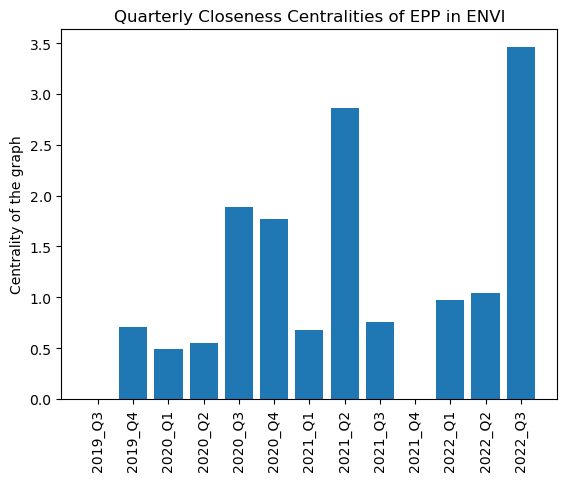
\includegraphics[height=3.5cm]{img/EPP_ENVI_Q_closeness.png}

	\pause \column{5cm}
	Closeness of S\&D in ENVI:
	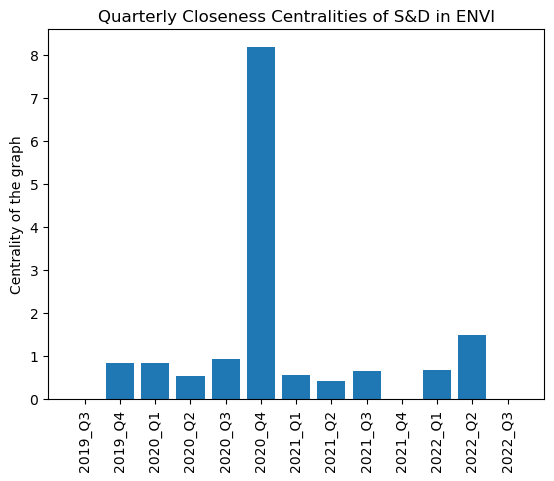
\includegraphics[height=3.5cm]{img/S&D_ENVI_Q_closeness.png}
	
	\end{columns}
\end{frame}

\begin{frame}
\frametitle{Our results: centrality}
	
	Considering the \bftext{closeness} centralities of parties in the \bftext{quarterly} and \bftext{committee} division and only in the \bftext{biggest component}:
	\vspace{4mm}
	\pause
	
	\begin{columns}
	\column{5cm}
	Closeness of EPP party in ITRE:
	\\
	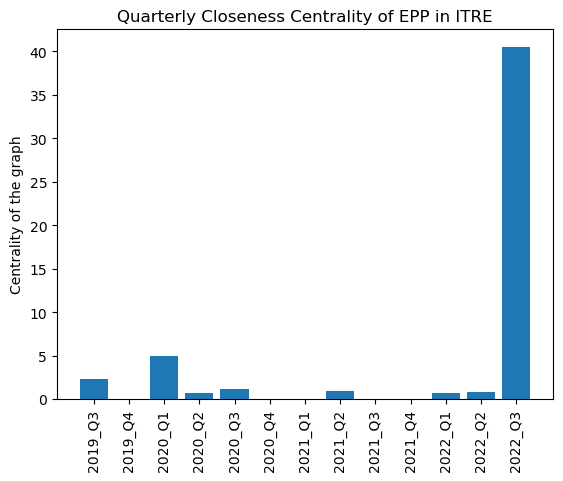
\includegraphics[height=3.5cm]{img/EPP_ITRE_Q_closeness.png}

	\pause \column{5cm}
	Closeness of S\&D in ITRE:
	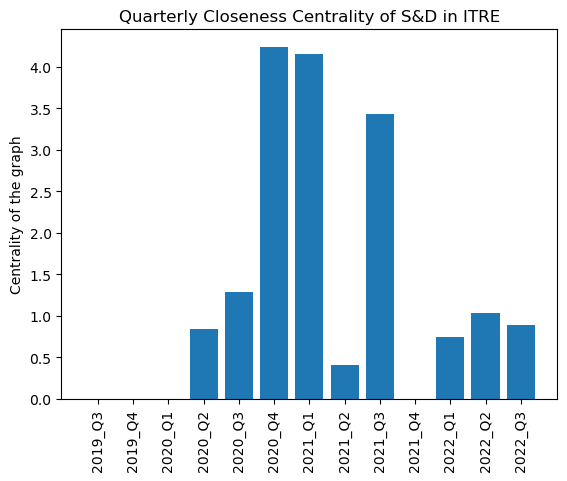
\includegraphics[height=3.5cm]{img/S&D_ITRE_Q_closeness.png}
	
	\end{columns}

\end{frame}

\begin{frame}
\frametitle{Our results: cohesion}
\end{frame}



\begin{frame}{}
	
	thx for watching
	
\end{frame}


\end{document}
